\section{Случайные процессы}

Речь пойдёт про процессы во времени, поведение которых нельзя однозначно предсказать: помехи сигналов, обучение моделей, курс валют и так далее.
Посмотрев на предысторию, необходимо построить модели, чтобы предсказать поведение процесса.

На основе теории вероятностей вводим параметр $t$ (время).

\begin{definition}{Случайный процесс}
    Параметрическое семейство случайных величин $\{\xi(\omega, t), ~ t \in T \subseteq \R\}$, определённых на одном вероятностном пространстве $(\Omega, \mathcal{F}, \mathbb{P})$, называется \textit{случайным процессом}.
\end{definition}

Встает вопрос о существовании такого объекта — рассмотрим позже.
Рассмотрим поведение процесса при фиксированных параметрах:
\begin{enumerate}
    \item Фиксируем $t_0$. Тогда $\xi(\omega, t_0)$ — это случайная величина. Это называется \textit{сечение} процесса в момент времени $t_0$.
    \item Фиксируем $\omega_0$. Тогда $\xi(\omega_0, t)$ — это детерминированная функция от $t$. Она называется \textit{траекторией} (или реализацией) случайного процесса.
\end{enumerate}

Две разных траектории процесса $\xi(t)$ для разных $\omega_0$ и $\omega_1$ могут иметь разное будущее, но общее прошлое и настоящее.

% TODO: Вставить рисунок с первой страницы (графики траекторий, расходящихся из одной точки)
\begin{figure}[h]
    \centering
    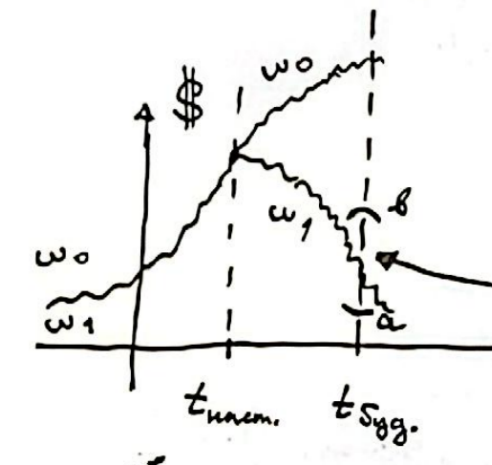
\includegraphics[width=0.3\textwidth]{images/placeholder_trajectories.png} 
    \caption{Траектории случайного процесса: разные исходы могут совпадать в прошлом, но различаться в будущем.}
    \label{fig:trajectories}
\end{figure}

Для того, чтобы вычислять вероятности событий, связанных с процессом, необходимо ввести функцию распределения для $\xi(\omega, t)$.
Для обычных случайных величин $F_{\xi}(x) = \mathbb{P}(\xi \le x)$, но для случайных процессов нужно рассмотреть семейство конечномерных распределений.

Пусть даны $n$ сечений: $\xi(\omega, t_1), ~ \xi(\omega, t_2), ~ \dots, ~ \xi(\omega, t_n)$, определённые на $(\Omega, \mathcal{F}, \mathbb{P})$. Тогда вектор $(\xi(\omega, t_1), \dots, \xi(\omega, t_n))$ определён на $(\Omega, \mathcal{F}, \mathbb{P})$ и его функция распределения имеет вид:

\begin{definition}{$n$-мерная функция распределения}
    Функция вида
    \[
        F_{\xi}(x_1, \dots, x_n; t_1, \dots, t_n) = \mathbb{P}(\omega : \{ \xi(t_1) \le x_1, \dots, \xi(t_n) \le x_n \})
    \]
    называется $n$-мерной функцией распределения процесса $\xi(\omega, t)$.
\end{definition}

\begin{definition}{Семейство конечномерных распределений}
    Совокупность таких функций распределения $\{F_{\xi}(x_1, \dots, x_n; t_1, \dots, t_n)\}$ для всех конечных наборов $\{t_1, \dots, t_n\} \subset T$ и всех $n \in \N$ называется \textit{семейством конечномерных распределений} процесса $\xi(\omega, t)$.
\end{definition}

Свойства (условия согласованности) семейства $\{F_{\xi}\}$:

\begin{enumerate}
    \item $0 \le F_{\xi}(x_1, \dots, x_n; t_1, \dots, t_n) \le 1$.
    \item $F_{\xi}(\dots)$ непрерывна справа по каждому аргументу $x_i$.
    \item Если хотя бы один $x_i \to -\infty$ (а остальные фиксированы), то $F_{\xi}(\dots) \to 0$.
    \item Если все $x_i \to +\infty$, то $F_{\xi}(\dots) \to 1$.
    \item \textit{Монотонность (неотрицательность меры прямоугольника):}
    Для любых $x_i, h_i > 0$ выполняется $\Delta F_{\xi} \ge 0$, где $\Delta$ — смешанная разность (аналог объема прямоугольника в $n$-мерном пространстве).
    \item \textit{Симметрия:} Для любой перестановки $k_1, \dots, k_n$ индексов $1, \dots, n$:
    \[
        F_{\xi}(x_{k_1}, \dots, x_{k_n}; t_{k_1}, \dots, t_{k_n}) = F_{\xi}(x_1, \dots, x_n; t_1, \dots, t_n).
    \]
    \item \textit{Согласованность:} Если устремить часть аргументов к $+\infty$, размерность распределения понижается:
    \[
        F_{\xi}(x_1, \dots, x_k, \underbrace{+\infty, \dots, +\infty}_{k+1, \dots, n}; t_1, \dots, t_n) = F_{\xi}(x_1, \dots, x_k; t_1, \dots, t_k).
    \]
\end{enumerate}

А что с вопросом о существовании?

\begin{theorem}{Теорема Колмогорова о существовании}
    Пусть задано семейство функций $F = \{ F(x_1, \dots, x_n; t_1, \dots, t_n) \}$, удовлетворяющее условиям $1)-7)$.
    Тогда существуют вероятностное пространство $(\Omega, \mathcal{F}, \mathbb{P})$ и случайный процесс $\{\xi(t), t \in T\}$ на нём, семейство конечномерных распределений которого совпадает с $F$.
\end{theorem}

\begin{note}{}
    \begin{enumerate}
        \item Случайный процесс $\xi(\omega, t)$ можно полностью задавать через семейство $F$.
        \item В теореме не гарантируется единственность процесса. Процессы надо как-то разделять/отождествлять.
    \end{enumerate}
\end{note}

\begin{definition}{Стохастическая эквивалентность}
    Случайные процессы $\{\xi(t), t \in T\}$ и $\{\eta(t), t \in T\}$ на $(\Omega, \mathcal{F}, \mathbb{P})$ называются \textit{стохастически эквивалентными}, если
    \[
        \forall t \in T \longmapsto \mathbb{P}(\omega : \{ \xi(\omega, t) = \eta(\omega, t) \}) = 1.
    \]
    При этом $\eta$ называется \textit{модификацией} $\xi$. Такие $\xi$ и $\eta$ обладают одними и теми же конечномерными распределениями.
\end{definition}

\subsection*{Выборочное пространство}

Можно рассматривать как исходы не просто $\omega$, а целые траектории $\xi(\omega, \cdot)$. Рассмотрим пространство функций $X^T = \{x(t) : T \to \mathbb{R}\}$, в котором лежат траектории процесса $\xi(t), t \in T$.

Введем $\sigma$-алгебру $\mathcal{B}_{X}^T$ подмножеств $X^T$, порождённую цилиндрическими множествами.

Цилиндрическое множество $C$ определяется как:
\[
    C = \{ x \in \mathbb{R}^T : x(t_1) \in B_1, \dots, x(t_n) \in B_n \}, \quad \text{где } B_i \in \mathcal{B}(\mathbb{R}).
\]
Это множества функций, проходящих через заданные «ворота» $B_i$ в моменты времени $t_i$.

% TODO: Вставить рисунок цилиндрического множества (график с воротами B1, B2, B3)
\begin{figure}[h]
    \centering
    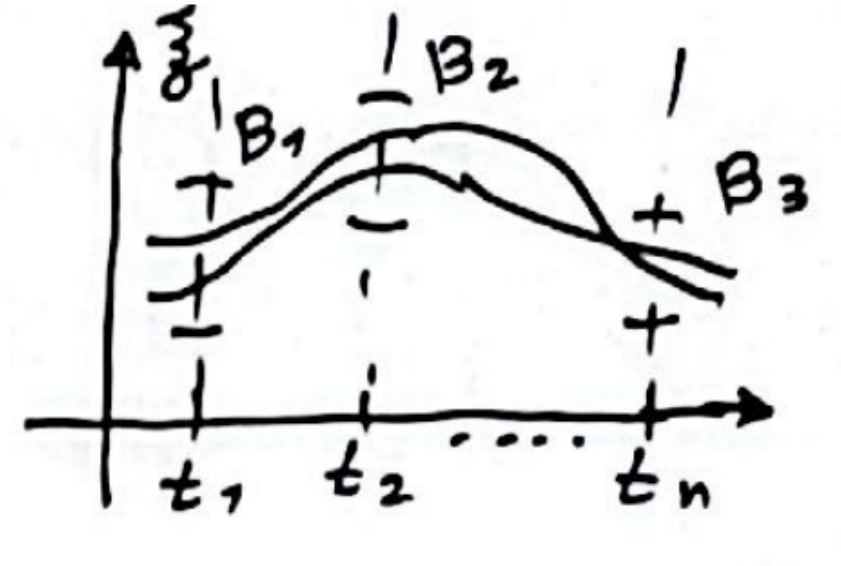
\includegraphics[width=0.3\textwidth]{images/placeholder_cylinders.png}
    \caption{Иллюстрация цилиндрического множества: траектории, проходящие через множества $B_1, B_2, B_3$ в моменты $t_1, t_2, t_3$.}
    \label{fig:cylinders}
\end{figure}

Отображение $\xi(\omega, t)$ определяет измеримое отображение $(\Omega, \mathcal{F}) \to (X^T, \mathcal{B}_{X}^T)$, так как прообраз любого цилиндрического множества лежит в $\mathcal{F}$.

Определим на $(X^T, \mathcal{B}_{X}^T)$ вероятностную меру:
\[
    P_{\xi}(B) = \mathbb{P}(\omega : \{ \xi(\omega, \cdot) \in B \}).
\]
В пространстве $(X^T, \mathcal{B}_{X}^T, P_{\xi})$ исход отождествляется с траекторией, а $P_{\xi}$ называется распределением процесса $\xi$.

Каким может быть множество $T$?
\begin{itemize}
    \item $T$ — 1 элемент $\Rarr$ Случайная величина.
    \item $T$ — конечно $\Rarr$ Случайный вектор.
    \item $T = \N, \mathbb{Z} \Rarr$ Случайная последовательность.
    \item $T = \R, \R_{+}, [a, b] \Rarr$ Случайный процесс.
\end{itemize}

Удобно считать $T = [a, b]$. Однако возникают проблемы с событиями, зависящими от несчётного числа моментов времени. Например, вероятность того, что процесс возрастает на участке $T$, или вероятности вида $\mathbb{P}(\sup_{t \in T} \xi(t) \le C)$.

\textbf{Пример проблемы:} пусть $\{\xi(t), t \ge 0\}$ определен на $(\Omega, \mathcal{F}, \mathbb{P})$. Пусть надо посчитать $\mathbb{P}(\sup_{t \in [0, 1]} \xi(t) \le x)$.
\[
    \{ \omega : \sup_{t \in [0, 1]} \xi(t) \le x \} = \bigcap_{t \in [0, 1]} \{ \xi(t) \le x \}.
\]
Для каждого $t$ событие $\{\xi(t) \le x\} \in \mathcal{F}$. Однако пересечение несчетного числа событий может не лежать в $\sigma$-алгебре $\mathcal{F}$.

Если предположить, что траектории непрерывны по $t$, тогда супремум по отрезку совпадает с супремумом по рациональным точкам:
\[
    \sup_{t \in [0, 1]} \xi(t) \le x \LRarr \sup_{t \in [0, 1] \cap \Q} \xi(t) \le x \LRarr \bigcap_{t \in [0, 1] \cap \Q} \{ \xi(t) \le x \} \in \mathcal{F}.
\]
Так как множество рациональных чисел $\Q$ счётно, пересечение счётно и событие измеримо.

\textbf{Вывод:} очень хорошо, когда траектории процесса непрерывные.

\begin{theorem}{Теорема Колмогорова о существовании непрерывной модификации}
    Пусть $\{\xi(t), t \in T\}$ — случайный процесс, $T = [a, b]$.
    Если существуют константы $\alpha > 0, ~ \beta > 0, ~ C < \infty$ такие, что для любых $t, t+h \in T$:
    \[
        \mathbb{E} |\xi(t+h) - \xi(t)|^{\alpha} \le C \cdot |h|^{1 + \beta},
    \]
    то процесс $\xi(t)$ имеет непрерывную модификацию $\eta(t)$.
\end{theorem}